\documentclass{article}

\usepackage[italian]{babel}
\usepackage[margin=2cm, footskip=5mm]{geometry}
% questi package non sono necessari in lualatex; ref https://tex.stackexchange.com/a/413046
% \usepackage[utf8]{inputenc}
% \usepackage[T1]{fontenc}
\usepackage{enumitem}
\usepackage{hyperref}
\usepackage{titlesec}
\usepackage{soulutf8}
\usepackage{contour}
\usepackage{float}
\usepackage{graphicx}
\usepackage{fancyhdr}
\usepackage{longtable}
\usepackage[table]{xcolor}
\usepackage{titling}
\usepackage{lastpage}
\usepackage{ifthen}
\usepackage{calc}
\usepackage{minted}
\usepackage{pgfgantt}
\usepackage{subfiles}

\newlength{\imgwidth}

\newcommand\scalegraphics[1]{%
    \settowidth{\imgwidth}{\includegraphics{#1}}%
    \setlength{\imgwidth}{\minof{\imgwidth}{\textwidth}}%
    \includegraphics[width=\imgwidth]{#1}%
}

% XXX definizione dei percorsi in cui cercare immagini
\graphicspath{ {./}
    {./img/}
}

% esempio di utilizzo: \appendToGraphicspath{./img/} (un comando diverso per ogni path da includere)
% N.B.: ci DEVE essere un forward slash alla fine del path, a indicare che è una cartella.
\makeatletter
\newcommand\appendToGraphicspath[1]{%
  \g@addto@macro\Ginput@path{{#1}}%
}
\makeatother

% setup della sottolineatura
\setuldepth{Flat}
\contourlength{0.8pt}

\newcommand{\uline}[1]{%
  \ul{{\phantom{#1}}}%
  \llap{\contour{white}{#1}}%
}

% setup dei link
\hypersetup{
  colorlinks=true, % set true if you want colored links
  linktoc=all,     % set to all if you want both sections and subsections linked
  linkcolor=black, % choose some color if you want links to stand out
}

% setup di header e footer
\pagestyle{fancy}

\fancyhf{}
\fancyhead[L]{\includegraphics[width=1cm]{logo.png}}
\fancyhead[R]{\thetitle}
\fancyfoot[R]{\thepage\ di~\pageref{LastPage}}

\fancypagestyle{nopage}{%
  \fancyfoot{}%
}

\setlength{\headheight}{1.2cm}

% setup forma \paragraph e \subparagraph
\titleformat{\paragraph}[hang]{\normalfont\normalsize\bfseries}{\theparagraph}{1em}{}
\titleformat{\subparagraph}[hang]{\normalfont\normalsize\bfseries}{\thesubparagraph}{1em}{}

% setup profondità indice di default
\setcounter{secnumdepth}{5}
\setcounter{tocdepth}{5}

% shortcut per i placeholder
\newcommand{\plchold}[1]{\textit{\{#1\}}} % chktex 20

% hook per lo script che genera il glossario
\newcommand{\glossario}[1]{\underline{#1}\textsubscript{g}}

% definizione dei comandi \uso e \stato
\makeatletter
\newcommand{\setUso}[1]{%
  \newcommand{\@uso}{#1}%
}
\newcommand{\uso}{\@uso}

\newcommand{\setStato}[1]{%
  \newcommand{\@stato}{#1}%
}
\newcommand{\stato}{\@stato}

\newcommand{\setVersione}[1]{%
  \newcommand{\@versione}{#1}%
}
\newcommand{\versione}{\@versione}

\newcommand{\setResponsabile}[1]{%
  \newcommand{\@responsabile}{#1}%
}
\newcommand{\responsabile}{\@responsabile}

\newcommand{\setRedattori}[1]{%
  \newcommand{\@redattori}{#1}%
}
\newcommand{\redattori}{\@redattori}

\newcommand{\setVerificatori}[1]{%
  \newcommand{\@verificatori}{#1}%
}
\newcommand{\verificatori}{\@verificatori}

\newcommand{\setDescrizione}[1]{%
  \newcommand{\@descrizione}{#1}%
}
\newcommand{\descrizione}{\@descrizione}

\newcommand{\setModifiche}[1]{%
  \newcommand{\@modifiche}{#1}%
}

\newcommand{\modifiche}{\@modifiche}

\makeatother

% setup delle description
\setlist[description,1]{font=$\bullet$\hspace{1.5mm}, labelwidth=* leftmargin=*,labelindent=12.5mm}
\setlist[description,2]{font=$\bullet$\hspace{1.5mm}, leftmargin=*,labelindent=12.5mm}

\appendToGraphicspath{../../commons/img/}

\title{Verbale esterno --- 13/01/2020}

\setResponsabile{Alessandro Rizzo}
\setRedattori{Alberto Cocco}
\setVerificatori{
  Tobia Apolloni \\ &
  Riccardo Cestaro
}
\setUso{Esterno}
\setDescrizione{Verbale dell'incontro di GruppOne del 13/01/2020}
\setModifiche{%
\cellcolor{white!80!lightgray!100} &Alessandro Rizzo & 2020--01--13 & approva documento \\%
\cellcolor{white!80!lightgray!100} &Tobia Apolloni, Riccardo Cestaro & 2020--01--13 & verifica verbale \\%
\multirow{-3}{*}{-} \cellcolor{white!80!lightgray!100} &Luca Ercole & 2020--01--13 & stendi verbale %
}

\disabilitaVersione{}
\disabilitaElencoFigure{}
\disabilitaElencoTabelle{}

\begin{document}

\thispagestyle{empty}
\pagenumbering{gobble}

\begin{center}

  \includegraphics[width=8.5cm]{\commons/img/logo.png}\\
  {\Large GruppOne - progetto "Stalker"}\\
  \vspace{1.5cm}

  {\Huge \thetitle}
  \vspace{1.5cm}

  \begin{table}[H]
    \centering

    \begin{tabular}{r|l}
      \textbf{Versione}     & \versione              \\
      \textbf{Approvazione} & \responsabile          \\
      \textbf{Redazione}    & \redattori             \\
      \textbf{Verifica}     & \verificatori          \\
      \textbf{Stato}        & \stato                 \\
      \textbf{Uso}          & \uso                   \\
      \textbf{Destinato a}  & Imola Informatica      \\
                            & GruppOne               \\
                            & Prof. Tullio Vardanega \\
                            & Prof. Riccardo Cardin  \\
    \end{tabular}
  \end{table}

  \vspace{3cm}
  \textbf{Descrizione}\\
  \descrizione\\
  \vfill
  \verb|gruppone.swe@gmail.com|
\end{center}

\newpage
\thispagestyle{nopage}

\section*{Registro delle modifiche}
\label{sec:registro_delle_modifiche}

\begin{table}[H]
  \label{tab:registro_delle_modifiche}

  \centering
  \rowcolors{2}{lightgray}{white!80!lightgray!100}

  \begin{longtable}[c]{c c c c l}
    \rowcolor{darkgray!90!}\color{white}{\textbf{Versione}} & \color{white}{\textbf{Data}} & \color{white}{\textbf{Nominativo}} & \color{white}{\textbf{Ruolo}} & \color{white}{\textbf{Descrizione}} \\\endhead
    \modifiche
  \end{longtable}
\end{table}

% section registro_delle_modifiche (end)
\newpage

\thispagestyle{nopage}
\pagenumbering{roman}
\tableofcontents

\newpage

\pagenumbering{arabic}


\section{Informazioni logistiche}%
\label{sec:informazioni_logistiche}

\begin{description}
  \item [Luogo] chiamata Hangouts
  \item [Data] 13/01/2020
  \item [Ora] 12:00 \symbol{8594} 13:30
\end{description}

\subsection{Membri del gruppo presenti}%
\label{sub:membri_del_gruppo_presenti}

\begin{enumerate}
  \item Riccardo Agatea
  % \item Tobia Apolloni
  \item Riccardo Cestaro
  \item Alberto Cocco
  \item Luca Ercole
  % \item Alberto Gobbo
  \item Alessandro Rizzo
  % \item Fabio Scettro
\end{enumerate}
% sub:membri_del_gruppo_presenti (end)

\subsection{Altri partecipanti}%
\label{sub:altri_partecipanti}
\begin{enumerate}
  \item Davide Zanetti (Imola Informatica, proponente del capitolato)
\end{enumerate}

% sub:altri_partecipanti (end)
% sec:informazioni_logistiche (end)

\section{Introduzione}%
\label{sec:introduzione}

In data 13/01/2020 presso il Dipartimento di Matematica ``Tullio Levi-Civita'' GruppOne si è collegato tramite una chiamata Hangouts al proponente. La riunione si è svolta sotto forma di discussione: ogni componente del gruppo ha inserito in un file Google Docs condiviso le domande che sono state poi sottoposte al proponente e sulle quali si è discusso. Segue una descrizione degli argomenti trattati.

\section{Ordine del giorno}%
\label{sec:ordine_del_giorno}

\begin{itemize}
  \item Modello incrementale.
  \item Configurazione del Server LDAP\@.
  \item Chiarimenti sulle modalità di autenticazione alle organizzazioni con tracciamento non anonimo.
  \item Metriche per la qualità di prodotto.
\end{itemize}

\section{Modello incrementale}%
\label{sec:modello_incrementale}

Abbiamo esposto al proponente la pianificazione del modello incrementale da noi adottato e gli abbiamo chiesto dei consigli su come strutturare la pianificazione di incrementi in un progetto così complesso. Il proponente ci ha consigliato, data la natura del prodotto, di identificare una prima fase in cui si definiscono i protocolli delle richieste tra la componente app e il server. In seguito ci ha consigliato di dividere il lavoro in flussi, ossia serie di azioni (traducibili in requisiti) che gli utenti possono effettuare, e dividere questi flussi tra gli incrementi di lunghezza fissa che abbiamo fissato, anche andando ad occupare più di un incremento per la realizzazione di un flusso.

\section{Configurazione del Server LDAP}%
\label{sec:obiettivi_in_uscita_alla_RQ}

Abbiamo chiesto al proponente specifiche maggiori sulla configurazione che l'owner di una organizzazione deve effettuare all'atto della creazione di una organizzazione. Il proponente ha chiarito che il server LDAP viene configurato per contenere le credenziali di accesso che in seguito gli utenti utilizzeranno per autenticarsi all'interno dell'organizzazione

\section{Chiarimenti sulle modalità di autenticazione alle organizzazioni con tracciamento non anonimo}%
\label{sec:chiarimenti_su_verifica}

Abbiamo presentato al proponente i nostri dubbi riguardo alla modalità di autenticazione degli utenti all'interno delle organizzazioni che la richiedessero. Il proponente ha ribadito che le credenziali vengono configurate dall'owner nel server LDAP e dunque è con quelle credenziali che gli utenti possono autenticarsi all'interno dell'organizzazione, sarà cura dell'owner fornire quelle credenziali alle persone autorizzate ad autenticarsi e il server LDAP garantirà loro l'accesso alle informazioni se le credenziali sono corrette.

\section{Metriche}%
\label{sec:metriche}

Abbiamo chiesto al proponente consigli su come decidere le metriche per la qualità di prodotto da inserire nelle norme di progetto. Il proponente ha accolto la nostra richiesta di chiarimenti ma ha rimandato a un secondo momento la sua risposta per fornirci indicazioni più specifiche al riguardo, contiamo di tenere in considerazione i suoi consigli e aggiornare di conseguenza le metriche per la qualità di prodotto.

\newpage
\section{Registro delle decisioni}%
\label{sec:registro_delle_decisioni}

\begin{description}
  \item[20200113-ext-001] abbiamo deciso di continuare con lo sviluppo del modello incrementale come già iniziato apportando delle modifiche per correlare ogni incremento con i flussi implementati.
  \item[20200113-ext-002] abbiamo perso la decisione di aggiornare il caso d'uso e i requisiti relativi all'autenticazione nelle organizzazioni per riflettere quanto richiesto dal proponente.
  \item[20200113-ext-003] terremo in considerazione i consigli che ci verranno forniti dal proponente e aggiorneremo di conseguenza le metriche per la qualità di prodotto.
\end{description}

% sec:registro_delle_decisioni (end)
\end{document}
